%Compile using xelatex
\documentclass[12pt]{article}
\usepackage{graphicx}
\usepackage{xltxtra,xgreek,fontspec} 
\usepackage{color}
\setmainfont{FreeSerif} % main font
\usepackage{setspace}
\usepackage[export]{adjustbox}[2011/08/13]
\usepackage[usenames,dvipsnames,svgnames,table]{xcolor}
\usepackage[textwidth=17cm]{geometry}
\usepackage[greek]{datetime2}
\usepackage{caption}
\captionsetup[figure]{name=Εικόνα, labelfont=it} % custom name for image description 
\usepackage{float}
\usepackage{fancybox}
\usepackage{changepage}
\usepackage{hyperref} % link customization
\hypersetup{
	colorlinks,
	linkcolor=black,
	citecolor={blue!50!black},
	urlcolor={blue!80!black}
}
\usepackage{tikz}
\usetikzlibrary{shadows}

\newcommand*\keystroke[1]{%
	\tikz[baseline=(key.base)]
	\node[%
	draw,
	fill=white,
	drop shadow={shadow xshift=0.25ex,shadow yshift=-0.25ex,fill=black,opacity=0.75},
	rectangle,
	rounded corners=2pt,
	inner sep=2pt,
	line width=0.5pt,
	font=\scriptsize\ttfamily
	](key) {#1\strut}
	;
}

\newfontfamily\myfont{GFS Didot} %custom font for university and dept. name
\usepackage{fancyhdr}
\pagestyle{fancy}
\fancyhf{}
\rhead{\footnotesize Σχεδίαση Δικτύων} % right header
\lhead{\footnotesize Lab 01: Εισαγωγή στο Cisco IOS} %left header
%\chead{\includegraphics[scale=0.25]{C:/uowm.png}}
\cfoot{\noindent\makebox[\linewidth]{\rule{0.75cm}{0.4pt}}\\\thepage} %custom page number format
\graphicspath{{./images/}}

\usepackage[flushmargin, hang, bottom]{footmisc}
\addtolength{\footnotesep}{2.5mm} % change to 1mm
\setlength{\parindent}{0pt}

\begin{document}
	
\begin{titlepage}
		
\newcommand{\HRule}{\rule{\linewidth}{0.5mm}} % Defines a new command for the horizontal lines, change thickness here
		
\centering % Center everything on the page

\includegraphics[scale=0.4]{icte-uowm}\\[1cm]
%----------------------------------------------------------------------------------------
%	HEADING SECTIONS
%----------------------------------------------------------------------------------------
		
\textsc{\Huge \myfont Πανεπιστήμιο Δυτικήσ Μακεδονίασ}\\[0.5cm] % University name
\textsc{\Large \myfont Τμήμα Μηχανικών Πληροφορικήσ και Τηλεπικοινωνιών}\\[0.5cm] % Department name
\large{Εργαστήριο Σχεδίασης Δικτύων}\\[0.1cm] % course title

%----------------------------------------------------------------------------------------
%	TITLE SECTION
%----------------------------------------------------------------------------------------
		
\HRule \\[0.5cm] {\LARGE \bfseries Lab 01: Εισαγωγή στο Cisco IOS}\\ % Lab title
\HRule \\[1.25cm]

%----------------------------------------------------------------------------------------
%	AUTHOR SECTION
%----------------------------------------------------------------------------------------
		
\begin{minipage}{0.85\textwidth}
	\myfont
	\begin{flushleft}
		\emph{Υπεύθυνος εργαστηρίου:}\\
		Όνομα \textsc{Επώνυμο}\\
	\end{flushleft}
\end{minipage}
						
\vfill % Fill the rest of the page with whitespace
						
%----------------------------------------------------------------------------------------
%	DATE SECTION
%----------------------------------------------------------------------------------------
						
{\large Κοζάνη, \today} % Date, change the \today to a set date if you want to be precise
						
\end{titlepage}

\section*{Πρόλογος}
Σκοπός του πρώτου εργαστηρίου είναι η εξοικείωση με τις συσκευές Cisco του εργαστηρίου, καθώς και η επισκόπηση βασικών εντολών για τον χειρισμό τους. \par
Το εργαστήριο προϋποθέτει βασικές γνώσεις ορολογίας Δικτύων Υπολογιστών, ειδικότερα όσον αφορά τα επίπεδα Ζεύξης Δεδομένων και Δικτύου.

\tableofcontents
\newpage

\section{Εργαστηριακός εξοπλισμός}

\subsection{Δομή Μεταγωγέα}
Τα μοντέλα των μεταγωγέων (switches) που θα χρησιμοποιηθούν στο πλαίσιο των εργαστηριακών ασκήσεων του μαθήματος είναι τα Cisco Catalyst 2960-SF και Cisco Catalyst 2960-X. 
\begin{figure}[H]
	\centering
	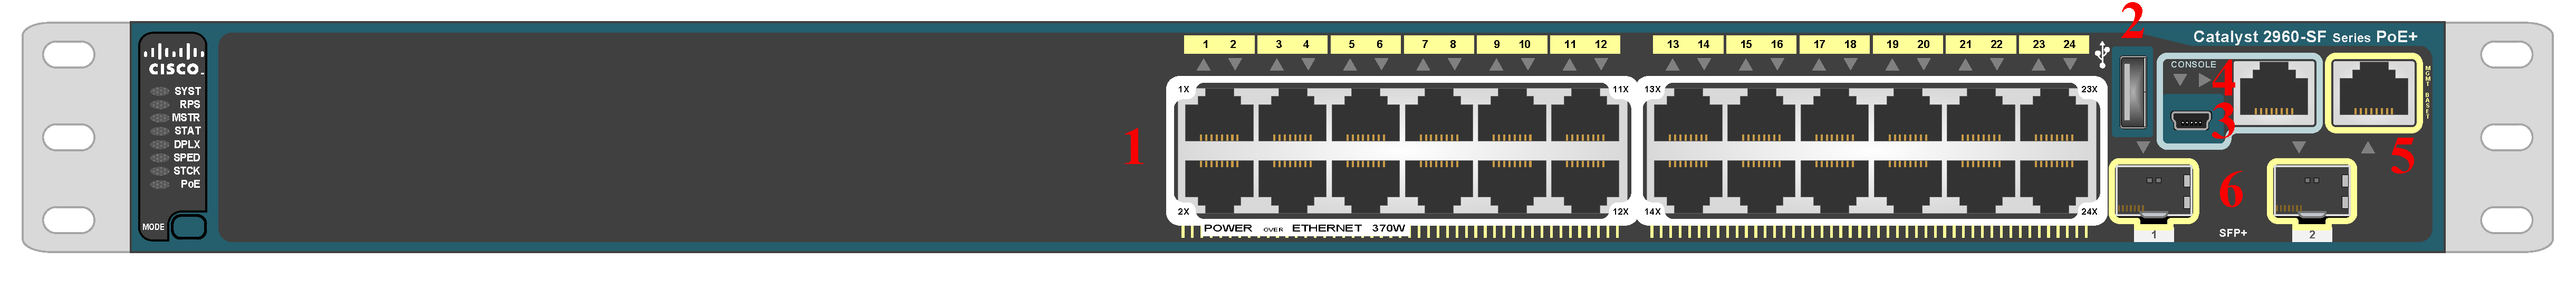
\includegraphics[scale=0.125]{c2960sf.jpg}
	\caption{\textit{Ο μεταγωγέας Cisco Catalyst 2960-SF}}
\end{figure}

Το Cisco Catalyst 2960-SF αποτελείται από τις εξής διεπαφές: 
\begin{enumerate}
	\setlength\itemsep{-0.1cm}
	\item 24 Fast Ethernet θύρες (10/100 Mbps) με υποστήριξη PoE+
	\item USB console θύρα
	\item RJ-45 console θύρα
	\item 2 MGMT (Fa0/0) Ethernet Management Port
	\item 2 θύρες Small Form-Factor Pluggable (SFP) ανόδου με υποστήριξη Gigabit
\end{enumerate}

\begin{figure}[H]
	\centering
	\includegraphics[scale=0.125]{c2960x-edited.jpg}
	\caption{\textit{Ο μεταγωγέας Cisco Catalyst 2960-X}}
\end{figure}
Το Cisco Catalyst 2960-X αποτελείται από τις εξής διεπαφές: 
\begin{enumerate}
	\setlength\itemsep{-0.1cm}
	\item 24 Gigabit Ethernet θύρες (10/100/1000 Mbps) με υποστήριξη PoE+
	\item USB console θύρα
	\item RJ-45 console θύρα
	\item 2 MGMT (Fa0/0) Ethernet Management Port
	\item 2 θύρες Small Form-Factor Pluggable (SFP) ανόδου με υποστήριξη Gigabit
\end{enumerate}

\subsection{Δομή Δρομολογητή}
\begin{figure}[H]
	\centering
	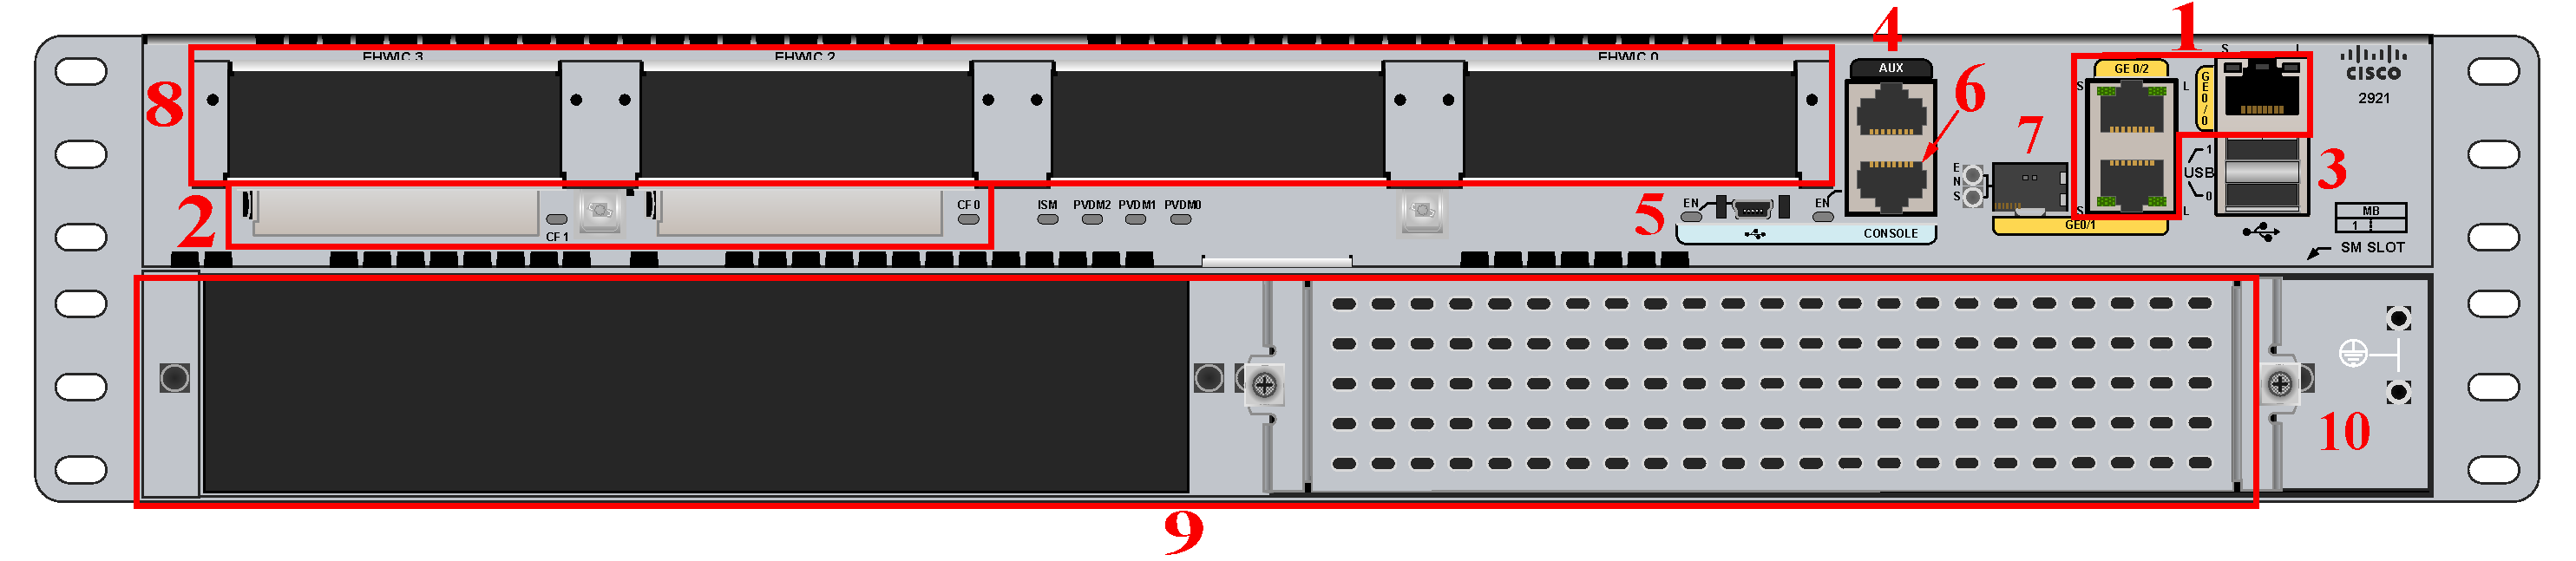
\includegraphics[scale=0.125]{c2921.jpg}
	\caption{\textit{Ο δρομολογητής Cisco Catalyst 2921}}
\end{figure}
Το μοντέλο του δρομολογητή του εργαστηρίου είναι το Cisco 2921, το οποίο αποτελείται από τις εξής διεπαφές:
\begin{enumerate}
	\setlength\itemsep{-0.1cm}
	\item 3 Gigabit Ethernet θύρες (10/100/1000 Mbps)
	\item USB \& RJ-45 console θύρες
	\item 2 θύρες Small Form-Factor Pluggable (SFP)
	\item 4 Cisco Enhanced High-Speed WAN Interface Cards (EHWIC)
	\item 2 Auxiliary Ports (AUX)
\end{enumerate} 

\section{Internetwork Operating System (IOS)}
To \textbf{Cisco IOS} είναι το λειτουργικό σύστημα που χρησιμοποιείται από τα μηχανήματα Cisco για την μεταγωγή και δρομολόγηση πακέτων, καθώς και για λειτουργίες διαδικτύωσης. Το ΛΣ παρέχει κατάλληλη διεπαφή χρήστη, η οποία επιτρέπει στον χρήστη την εκτέλεση εκατοντάδων εντολών για τον έλεγχο της συσκευής του.

\subsection{Διεπαφή Χρήστη}
Το \textbf{IOS Tcl} (Tool Command Language) είναι η βασική διεπαφή γραμμής εντολών, η οποία προσφέρει ένα πακέτο από εντολές πολλών λέξεων. Το διαθέσιμο σετ εντολών αποφασίζεται και εξαρτάται από την κατάσταση (mode) και τα δικαιώματα του εκάστοτε χρήστη.\par 
Σε όλες τις εντολές εκχωρείται ένα προνομιακό επίπεδο (privilege level) από το 0 μέχρι το 15 και μπορούν να προσπελαστούν μόνο από χρήστες με τα απαραίτητα προνόμια. Τα διαθέσιμα command modes είναι τα εξής:
\begin{itemize}
	\item \textbf{User EXEC Mode} (>)\\
	H προεπιλεγμένη κατάσταση κατά την σύνδεση του χρήστη στο μηχάνημα.
	\item \textbf{Privileged EXEC Mode} (\#)\\
	Κατάσταση επαυξημένων δικαιωμάτων, στην οποία γίνονται περισσότερες εντολές διαθέσιμες.
	\item \textbf{Global Configuration Mode} (\texttt{conf})\\
	Προσφέρει εντολές για τις βασικές ρυθμίσεις του συστήματος.
	\item \textbf{Interface Configuration Mode} (\texttt{conf-if})\\
	Προσφέρει εντολές για τις ρυθμίσεις μιας συγκεκριμένης διεπαφής.
	\item ROM Monitor Mode
	\item Setup Mode
	\item Παραπάνω από 100 configuration modes και submodes.
\end{itemize}
Δίπλα από το όνομα του κάθε command mode παρατίθεται το σύμβολο ή η λέξη κλειδί που την διακρίνει. Εμφανίζεται πάντα στο prompt της γραμμής εντολών, δίπλα από το όνομα της συσκευής. Με αυτό τον τρόπο ο χρήστης γνωρίζει κατευθείαν την κατάσταση στην οποία βρίσκεται και τι εντολές έχει διαθέσιμες.

\subsection{Μνήμες}
Οι συσκευές Cisco χρησιμοποιούν τα εξής είδη μνήμης:
\begin{itemize}
	\item[\textbf{ROM}:] Στην μνήμη αυτή αποθηκεύεται το bootstrap του συστήματος, δηλαδή το αρχικό λογισμικό που εκτελείται κατά την εκκίνηση του ΛΣ.
	\item[\textbf{Flash}:] Περιέχει μια ή περισσότερες εκδόσεις του IOS, οι οποίες μπορούν να χρησιμοποιηθούν για αναβάθμιση. Επίσης, χρησιμοποιείται για την αποθήκευση αρχείων ρυθμίσεων και πληροφοριών συστήματος.
	\item[\textbf{RAM}:] Πρόκειται για τον γνωστό τύπο μνήμης τυχαίας προσπέλασης που χρησιμοποιείται και στους υπολογιστές. Στα μηχανήματα Cisco χρησιμοποιείται για την αποθήκευση προσωρινών πινάκων δρομολόγησης και πακέτων προς δρομολόγηση ή προς ανάλυση της λογικής τους διεύθυνσης. Επίσης, περιέχει το αρχείο running configuration.
	\item[\textbf{NVRAM}:] Σε αυτή την μνήμη αποθηκεύονται οι ρυθμίσεις εκκίνησης (startup configuration). Κατά την εκκίνησή του, το IOS διαβάζει το αρχείο που βρίσκεται σε αυτή την μνήμη για την σωστή αρχικοποίηση του. Λόγω του ρόλου της, η μνήμη αυτή είναι ιδιαίτερα γρήγορη.
\end{itemize}

\subsection{Αποθήκευση ανάκτηση και επαναφορά ρυθμίσεων}
Κάθε φορά που γίνονται αλλαγές στις ρυθμίσεις της συσκευής, αυτές θα πρέπει να αποθηκεύονται στην NVRAM, ούτως ώστε να μην χαθούν κατά το reboot. Υπάρχουν δύο ειδών αρχεία ρυθμίσεων: το \textbf{running} (current operating) \textbf{configuration} και τo \textbf{startup configuration}.\\\newline
Για να εμφανίσετε τις τρέχουσες ρυθμίσεις (running configuration) μπορείτε να εκτελέσετε την εντολή:

\begin{flushleft}
	\ovalbox{\texttt{Router\# show running-config}}
\end{flushleft}

Η αποθήκευση των running configurations στο startup configuration file στην NVRAM γίνεται με την εντολή:

\begin{flushleft}
	\ovalbox{\texttt{Router\# copy running-config startup-config}}
\end{flushleft}

Για να εμφανίσετε τις startup configuration μπορείτε να εκτελέστε την εντολή: 

\begin{flushleft}
	\ovalbox{\texttt{Router\# show startup-config}}
\end{flushleft}

Για να χρησιμοποιείσετε τις startup configuration ως running-configuration: 

\begin{flushleft}
	\ovalbox{\texttt{Router\# copy startup-config running-config}}\\
\end{flushleft}

Για να διαγράψετε και τα δύο configuration files, δηλαδή να επαναφέρετε το μηχάνημα στις εργοστασιακές ρυθμίσεις, μπορείτε να συνδυάσετε τις εντολές \texttt{write erase} και \texttt{reload}.\\

\begin{Sbox}
	\begin{minipage}{4in}
		\texttt{Router\# write erase\\
			Router\# reload}
	\end{minipage}
\end{Sbox}
\fbox{\TheSbox}
\\

Στις ερωτήσεις "\texttt{System configuration has been modified. Save?}" και "\texttt{Would you like to enter the initial configuration dialog?}" απαντάτε \texttt{no}.\\

Επίσης, μπορείτε να επαναφέρετε τις εργοστασιακές ρυθμίσεις της συσκευής σας πατώντας παρατεταμένα (8-9 δευτερόλεπτα) το κουμπί mode στην μπροστά πρόσοψη του μηχανήματος.

\begin{figure}[H]
	\centering
	\includegraphics[scale=0.5]{reset-button.jpg}
	\caption{\textit{To κουμπί mode, κάτω από τις φωτεινές ενδείξεις της συσκευής}}
\end{figure}

\subsection{Απαρίθμηση διεπαφών}
Σε κάθε διεπαφή Ethernet έχει ανατεθεί μια ονομασία της μορφής:

\begin{center}
	\texttt{\large PorttypeΧ/Υ/Z}\hspace*{0.5cm} ή\hspace*{0.5cm} \texttt{\large PorttypeΧ/Z}
\end{center}

Το \texttt{Χ} αριθμός αφορά το slot στο οποίο βρίσκεται η θύρα, το \texttt{Y} το subslot και το \texttt{Z} τον μοναδικό αριθμό της θύρας για το slot ή το slot/subslot που αυτή βρίσκεται. Το \texttt{Porttype} είναι ένα keyword που δηλώνει την τεχνολογία της θύρας, η οποία μπορεί να είναι \texttt{FastEthernet} (\texttt{Fa}), \texttt{GigabitEthernet} (\texttt{Gi} ή \texttt{Ge}) ή \texttt{TenGigabitEthernet}. Η ονομασία \texttt{PorttypeΧ/Υ/Z} χρησιμοποιείται σε εντολές στο Cisco IOS προκειμένου να αναφερθούμε στην αντίστοιχη θύρα του μηχανήματος.

\section{Βασικές εντολές του Cisco IOS}
H ενότητα αυτή παραθέτει μερικές από τις πιο βασικές εντολές για την διαχείριση \textbf{οποιασδήποτε} συσκευής Cisco. Οι εντολές αυτές, δηλαδή, μπορούν να εκτελεστούν και σε δρομολογητές και σε μεταγωγείς.

\subsection{Login στο κέλυφος της συσκευής}
Αρχικό βήμα για τον χειρισμό της συσκευής Cisco είναι η σύνδεση σε αυτή. Η σύνδεση πραγματοποιείται μέσω θύρας COM, με την χρήση του προγράμματος PuTTY, το οποίο ρυθμίζεται όπως στην παρακάτω εικόνα:

\begin{figure}[H]
	\centering
	\includegraphics[scale=0.75]{login1}
\end{figure}

Στο κενό παράθυρο του PuTTY που εμφανίζεται θα πρέπει να πατήσετε μια φορά το \keystroke{Enter} για να εμφανιστεί το command prompt. 

\begin{figure}[H]
	\centering
	\includegraphics[scale=0.75]{login2}
\end{figure}

\subsection{Προβολή βοήθειας}
Με την εντολή \ovalbox{\texttt{help}} ακολουθούμενη από το όνομα μιας εντολής μπορείτε να εκκινήσετε την υπηρεσία βοήθειας που παρέχει το Cisco IOS και να προβάλλετε χρήσιμες πληροφορίες για την εντολή που σας ενδιαφέρει.
\begin{figure}[H]
	\centering
	\includegraphics[scale=.75]{help}
\end{figure}

\subsection{Μετάβαση σε privileged mode}
Για να μεταβείτε σε privileged mode αρκεί να εκτελέσετε την εντολή \ovalbox{\texttt{enable}} και μετά να πληκτρολογήσετε τον κωδικό πρόσβασης. Αυτός παρέχεται από τους υπεύθυνους του εργαστηρίου. Αναγνωρίζετε πως είστε σε κατάσταση privileged διακρίνοντας την δίεση (\#) στο command prompt, η οποία αντικαθιστά το σύμβολο συγκρίσεως (>).
\begin{figure}[H]
	\centering
	\includegraphics[scale=.75]{privileged}
\end{figure}
Εξέρχεστε από την προνομιακή κατάσταση με την εντολή \ovalbox{\texttt{disable}}.

\subsection{Συντομεύσεις εντολών/πληκτρολογίου}
Το IOS δίνει την δυνατότητα στον χρήστη να εκτελέσει μια εντολή πληκτρολογώντας τον ελάχιστο αριθμό χαρακτήρων που την προσδιορίζουν μοναδικά. Για να δείτε σε ποιες εντολές αντιστοιχεί μια συντόμευση, μπορείτε να πληκτρολογήσετε το επιθυμητό πλήθος χαρακτήρων, ακολουθούμενο από το ερωτηματικό.
Για παράδειγμα, η εντολή \texttt{con?} επιστρέφει δυο δυνατές επιλογές, την \texttt{configure} και την \texttt{connect}. Συνεπώς, η \texttt{conf?} επιστρέφει μόνο την \texttt{configure}. Εκτελώντας, λοιπόν, την εντολή \texttt{conf} είναι σαν να εκτελείτε την εντολή \texttt{configure}.

\begin{figure}[H]
	\centering
	\includegraphics[scale=.75]{conf}
\end{figure}
Επίσης, συντομεύσεις μπορούν να χρησιμοποιηθούν και για διάφορα keywords, όπως ο τύπος μιας θύρας. Για παράδειγμα, μπορείτε να αναφερθείτε στην θύρα \texttt{GigabitEthernet1/0/1} γράφοντας μόνο \texttt{Gi1/0/1}.\\

Παρακάτω δίνεται ένας συνοπτικός πίνακας με τις συντομεύσεις πληκτρολογίου για ευκολότερη πρόσβαση/διαχείριση της δικτυακής συσκευής:
\begin{center}
\begin{tabular}{ll}
	\textbf{Συντόμευση}&\textbf{Αποτέλεσμα} \\\hline
	\keystroke{Ctrl} + \keystroke{P} ή \keystroke{$\ \uparrow\ $} & Εμφάνιση τελευταίας εντολής που δόθηκε\\
	\keystroke{Ctrl} + \keystroke{N} ή \keystroke{$\ \downarrow\ $} & Εμφάνιση προηγούμενων εντολών που δόθηκαν\\
	\keystroke{Ctrl} + \keystroke{A} & Μετακίνηση κέρσορα στην αρχή της γραμμής\\
	\keystroke{Ctrl} + \keystroke{E} & Μετακίνηση κέρσορα στο τέλος της γραμμής\\
	\keystroke{Esc } + \keystroke{B} & Μετακίνηση κέρσορα προς τα πίσω κατά μια λέξη\\
	\keystroke{Esc } + \keystroke{F} & Μετακίνηση κέρσορα προς τα εμπρός κατά μια λέξη\\
	\keystroke{Ctrl} + \keystroke{R} & Επανεμφάνιση μιας γραμμής\\
	\keystroke{Ctrl} + \keystroke{U} & Διαγραφή μιας γραμμής\\
	\keystroke{Ctrl} + \keystroke{W} & Διαγραφή μιας λέξης\\
	\keystroke{Ctrl} + \keystroke{Z} & Τερματισμός της κατάστασης ρυθμίσεων και επιστροφή στην κατάσταση EXEC\\
	\keystroke{Tab} & Ολοκλήρωση της πληκτρολόγησης μιας εντολής
\end{tabular}
\end{center}

\subsection{Κατάσταση ρυθμίσεων}
Για να εφαρμόσετε βασικές ρυθμίσεις στην δικτυακή συσκευή θα πρέπει να μεταβείτε σε configuration mode. Αυτό μπορεί να γίνει με την εντολή \ovalbox{\texttt{conf}} ή \ovalbox{\texttt{configure}}. Αναγνωρίζετε πως είστε σε κατάσταση configuration βλέποντας την ένδειξη config στα αριστερά της δίεσης στο command prompt.

\begin{figure}[H]
	\centering
	\includegraphics[scale=.75]{conf-mode}
\end{figure}

Η εφαρμογή ρυθμίσεων μπορεί να γίνει είτε μέσω του τερματικού είτε μέσω δικτύου. Ο εξοπλισμός που διαθέτετε έχει στηθεί για ρύθμιση μέσω τερματικού, συνεπώς για να μεταβείτε σε configuration mode θα δίνετε την εντολή \ovalbox{\texttt{configure terminal}} ώστε κατευθείαν να προσδιορίσετε πως θα εφαρμόσετε ρυθμίσεις μέσω τερματικού.\\
Για να εξέλθετε από την κατάσταση ρυθμίσεων μπορείτε να δώσετε την εντολή \ovalbox{\texttt{exit}} ή τον συνδυασμό πλήκτρων \keystroke{Ctrl} + \keystroke{Z}.

\subsection{Αλλαγή κωδικού πρόσβασης}
Για να αλλάξετε τον κωδικό πρόσβασης του privileged mode θα πρέπει, αφού είστε ήδη σε αυτό το mode, εκτελείτε την εντολή \ovalbox{\texttt{enable secret pass}}, όπου \texttt{pass} ο επιθυμητός κωδικός πρόσβασης, και έπειτα την εντολή \ovalbox{\texttt{exit}} για να εξέλθετε από το configuration mode και να αποθηκευτούν οι αλλαγές.

\begin{figure}[H]
	\centering
	\includegraphics[scale=.75]{set-new-pass}
\end{figure}

\subsection{Αλλαγή hostname}
Για να αλλάξετε το όνομα της συσκευής θα πρέπει, αφού μεταβείτε σε config mode, να εκτελέσετε την εντολή \ovalbox{\texttt{hostname new\_hostname}}, όπου \texttt{new\_hostname} το νέο όνομα της δικτυακής οντότητας.

\begin{figure}[H]
	\centering
	\includegraphics[scale=.75]{hostname}
\end{figure}

\subsection{Διαχείριση φακέλων}
\begin{center}
	\begin{tabular}{ll}
		\textbf{Εντολή} & \textbf{Αποτελέσματα} \\\hline
		 \texttt{pwd} & Εμφάνιση τρέχοντος καταλόγου εργασίας\\
		 \texttt{dir} & Εμφάνιση περιεχομένων ενός καταλόγου \\
		 \texttt{mkdir} & Δημιουργία νέου καταλόγου \\
		 \texttt{rmdir} & Διαγραφή ενός καταλόγου\\
		 \texttt{cd} & Αλλαγή τρέχοντος καταλόγου εργασίας\\
		 \texttt{show file} & Εμφάνιση πληροφοριών για συγκεκριμένο κατάλογο ή αρχείο\\
		 \texttt{delete} & Διαγραφή ενός αρχείου\\
		 \texttt{more} & Προβολή περιεχομένων ενός αρχείου
	\end{tabular}
\end{center}

\subsection{Προβολή πληροφοριών}
Με την εντολή \ovalbox{\texttt{Router\# show interface}} μπορείτε να προβάλλετε αναλυτικές λεπτομέρειες για όλες τις δικτυακές διεπαφές της συσκευής που χειρίζεστε.\\\par

Μπορείτε να περιορίσετε τα αποτελέσματα της εντολής ορίζοντας το όνομα της διεπαφής που σας ενδιαφέρει. Για παράδειγμα, η εντολή \ovalbox{\texttt{Router\# show interface GigabitEthernet1/0/1}} θα εμφανίσει πληροφορίες για την διεπαφή \texttt{GigabitEthernet1/0/1}.
\begin{figure}[H]
	\centering
	\includegraphics[scale=.75]{show-spec-interface}
\end{figure}

Πολύ χρήσιμη είναι η εντολή \ovalbox{\texttt{Router\# show ip interface brief}}, η οποία προβάλλει μια σύνοψη της κατάστασης όλων των διεπαφών της συσκευής. Συγκεκριμένα, για κάθε διεπαφή διακρίνετε αν είναι ενεργοποιημένη και αν έχει αντιστοιχηθεί IP διεύθυνση σε αυτήν.
\begin{figure}[H]
	\centering
	\includegraphics[scale=.75]{show-ip-brief}
\end{figure}

Τέλος, με την εντολή \ovalbox{\texttt{Router\# show version}} μπορείτε να δείτε πληροφορίες που αφορούν την δικτυακή σας συσκευή, όπως έκδοση IOS, χαρακτηριστικά του hardware κ.λ.π.

\subsection{Διασωλήνωση}
Με την χρήση της διασωλήνωσης (\texttt{|}) μπορείτε να φιλτράρετε τα αποτελέσματα μιας εντολής. Για παράδειγμα:\\[0.25cm]
\begin{tabular}{lp{8cm}}
	\textbf{Εντολή} & \textbf{Αποτέλεσμα} \\\hline
	\texttt{sh running-config | ?} & Εμφάνιση όλων των δυνατών επιλογών για την εντολή διασωλήνωσης, όπως \texttt{begin}, \texttt{include}, \texttt{exclude} κ.τ.λ. \\[0.25cm]
	\texttt{sh run | begin interface} & Εμφάνιση τρέχουσας κατάστασης ρυθμίσεων ξεκινώντας από τις ρυθμίσεις των διεπαφών.\\[0.25cm]
	\texttt{show ip route | include 192.168.3.32} & Εμφάνιση όλων των καταχωρήσεων του πίνακα δρομολόγησης, οι οποίες περιλαμβάνουν την διεύθυνση \texttt{192.168.3.32}.
\end{tabular}

\subsection{MOTD banner}

Με την εντολή \texttt{banner motd} μπορείτε να ορίσετε το μήνυμα-της-ημέρας (MOTD - Message Of The Day), το οποίο προβάλλεται όταν ένας χρήστης συνδέεται σε ένα μηχάνημα Cisco. Η εντολή είναι διαθέσιμη στο configuration mode και η γενική της μορφή είναι η εξής:\\

\begin{Sbox}
	\begin{minipage}{4in}
		\texttt{\texttt{banner motd} delimiter message delimiter}
	\end{minipage}
\end{Sbox}
\fbox{\TheSbox}\\

Όπου \texttt{message}, το μήνυμα που επιθυμούμε να προβάλλεται στον χρήστη και \texttt{delimiter} ένας χαρακτήρας, εκτός από \texttt{"} και \texttt{\%}, ο οποίος δηλώνει την έναρξη και το τέλος του μηνύματος και δεν περιέχεται μέσα στο μήνυμα. Ένα παράδειγμα εκτέλεσης φαίνεται στην παρακάτω εικόνα:
\begin{figure}[H]
	\centering
	\includegraphics[scale=.75]{motd}
\end{figure}

Για να δημιουργήσετε ένα banner πολλών γραμμών, πιέστε \keystroke{Enter} πριν πληκτρολογήσετε τον δεύτερο \texttt{delimeter} ώστε να εισάγετε νέα γραμμή. 

\par Τέλος, η επαναφορά του banner στην προεπιλογή γίνεται με την παρακάτω εντολή:\\
 
\begin{Sbox}
	\begin{minipage}{4in}
		\texttt{Router(config)\# no banner motd}
	\end{minipage}
\end{Sbox}
\fbox{\TheSbox}

\subsection{Απενεργοποίηση domain-lookup}

Όταν δίνεται για εκτέλεση μια εντολή η οποία δεν αναγνωρίζεται από το Cisco IOS, τότε αυτό μπορεί να υποθέσει ότι η άγνωστη εντολή είναι ένα όνομα τομέα (domain name), με αποτέλεσμα να ξεκινήσει διαδικασία αναζήτησης για αυτό. Γιαυτό το λόγο, συνήθης τακτική κατά την διάρκεια ρύθμισης δικτυακών συσκευών Cisco είναι η απενεργοποίηση της λειτουργίας αναζήτησης ονομάτων τομέα, η οποία μπορεί να επιτευχθεί με την εντολή:

\begin{flushleft}
	\ovalbox{\texttt{Router(conf)\# no ip domain-lookup}}
\end{flushleft}

\subsection{Εντολή no}
Με την γενικής χρήσης εντολή \texttt{no} μπορείτε να ακυρώσετε την ενέργεια που προκαλεί η εντολή που την ακολουθεί.\\

Για παράδειγμα, η εντολή \ovalbox{\texttt{ip routing}} έχει ως αποτέλεσμα την ενεργοποίηση της λειτουργίας της δρομολόγησης πακέτων σε έναν δρομολογητή. Η απενεργοποίηση της λειτουργίας της δρομολόγησης σε έναν δρομολογητή γίνεται πολύ απλά με την εντολή \ovalbox{\texttt{no ip routing}}. Η χρήση της εντολής \texttt{no} θα γίνει πιο κατανοητή στην πράξη σε επόμενα εργαστήρια.


\end{document}